\documentclass[11pt]{article}
\usepackage[margin=1in]{geometry} 
\usepackage{amsmath,amsthm,amssymb,amsfonts}
\usepackage{color}
\usepackage[usenames,dvipsnames]{xcolor} % allows you to use color names, call this BEFORE you call TikZ
\usepackage{tikz, tikz-3dplot, pgfplots, tkz-graph}
\usetikzlibrary{patterns, positioning}  % allows you to use silly patterns as fill
\usepackage{marvosym} % a large repertoire of symbols
\usepackage{fancyhdr}
\pagestyle{fancy}
\lhead{\textbf{2D Graphing Master Document}}
\chead{}
\rhead{}
\lfoot{}
\cfoot{}
\rfoot{\thepage}
\renewcommand{\headrulewidth}{0.4pt}
\renewcommand{\footrulewidth}{0.4pt}


%%%%%%%%%%%%%%%%%%%%%%%%%%%%%%%%%%%%%%%%%%%%%%%%%%%%%%%%%%%%%%%%%%%%%%%%%%%%%%%%%%%%%%%%%%%%%%%%%%%%%%%%%%
%%%%%%%  This allows me to draw vertical asymptotes inside an axis environment using vasymptote=c  %%%%%%%
\pgfplotsset{vasymptote/.style={
    before end axis/.append code={
        \draw[dashed] ({rel axis cs:0,0} -| {axis cs:#1,0})
        -- ({rel axis cs:0,1} -| {axis cs:#1,0});
    }
}}
%%%%%%%%%%%%%%%%%%%%%%%%%%%%%%%%%%%%%%%%%%%%%%%%%%%%%%%%%%%%%%%%%%%%%%%%%%%%%%%%%%%%%%%%%%%%%%%%%%%%%%%%%%



% Sets version of pgfplots
\pgfplotsset{compat=1.9, samples=200} %%% Set samples to 200 for printing. Set it to lower for faster compiling.

% Zero indentation
\setlength\parindent{0pt}

    
    
    
\begin{document}
 
Here is a graph with many features.
  \begin{center}
   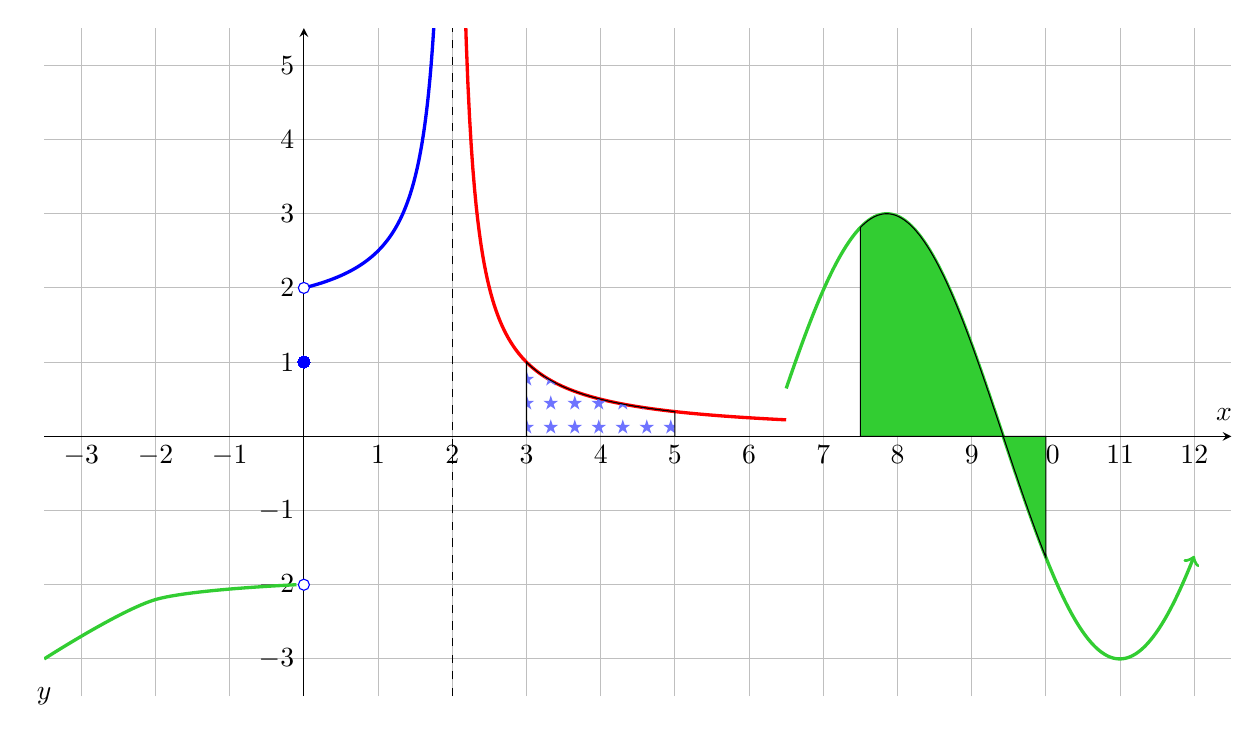
\begin{tikzpicture}
    \begin{axis}[ 
        scale=2.2,
	xmin=-3.5, xmax=12.5,
	ymin=-3.5, ymax=5.5,
	xtick={-3,...,12}, ytick={-3,...,5},
	major tick length={0},
	grid=major,               % change this to ``none'' to turn off the grid
	axis lines=center,
	axis equal image,         % This makes the grid square
	vasymptote=2              % vertical asymptote
	] 
	% Plot a smooth graph by picking points
	\addplot[very thick, smooth, color=LimeGreen, mark=none] plot coordinates{(-3.5,-3)(-2,-2.2)(-.1,-2)};
	
	% Plot a piecewise function by specifying the domain
	\addplot[very thick, color=blue, domain=0:1.9] {-1/(x-2)+1.5};
	
	% Fill the graph with stars! (See p.393 of the TikZ manual for more patterns)
	\addplot[very thick, color=red, domain=2.1:6.5] {1/(x-2)};
	\addplot [pattern=fivepointed stars, pattern color=Periwinkle, domain=3:5] {1/(x-2)} \closedcycle;
	
	% Fill the graph with green!
	\addplot[very thick, color=LimeGreen, domain=6.5:12, ->] {3*sin(deg(x))};
	\addplot [fill=LimeGreen, domain=7.5:10] {3*sin(deg(x))} \closedcycle;
	
	% Make filled-in dots
	\addplot [only  marks, mark=*, mark options={scale=1}, color=blue] (0,1);
	
	% Make white-filled open dots
	\addplot [only  marks, mark=*, mark options={scale=1, fill=white}, color=blue,] plot coordinates{(0,2)(0,-2)};
	
	% Draw on the graph using coordinates of the axes. You can only draw inside axes with this.
	\node at (axis cs:12.4,.3) {$x$};
	
    \end{axis}
    
        % Draw on picture using lower left as (0,0). You can draw outside axes with this.
        \draw (0,0) node{$y$};
        
        
   \end{tikzpicture}
  \end{center}


\end{document}
